\documentclass[12pt, oneside]{amsart}

\usepackage{amssymb}
\usepackage[
    style=numeric-comp,
    backend=biber,
    sorting=nty,
    doi=false,
    isbn=false, 
    natbib=true]{biblatex}
\addbibresource{references.bib}
\emergencystretch=1em

\usepackage{mathtools}
\usepackage{xcolor}
\usepackage{url} % Makes urls nicer
\usepackage[breaklinks=true]{hyperref}
\usepackage{cleveref}

% For tabular
\usepackage{booktabs}
\usepackage{array}
\usepackage{adjustbox}
\usepackage{multirow}
\usepackage{makecell}

% For figures
\usepackage{graphicx}

% Floating for positioning environments
\usepackage{float}


\newtheorem{thm}{Theorem}[section]
\newtheorem{prop}[thm]{Proposition}
\newtheorem{lem}[thm]{Lemma}
\newtheorem{cor}[thm]{Corollary}

\theoremstyle{definition}
\newtheorem{definition}[thm]{Definition}

\theoremstyle{remark}
\newtheorem{remark}[thm]{Remark}

\numberwithin{equation}{section}


% Package specific things

% TODO: Do we want to have equations just labeled with "(3.1)" or with 
% TODO: "equation 3.1".
%\crefname{equation}{equation}{equations} 
%\Crefname{equation}{Equation}{Equations}
\crefname{equation}{}{} 
\Crefname{equation}{}{}

\crefname{table}{table}{tables}
\Crefname{table}{Table}{Tables}

\crefname{figure}{figure}{figures}
\Crefname{figure}{Figure}{Figures}


% Definitions
\newcommand{\defn}{\ensuremath{:=}}
\newcommand{\revdefn}{=:}

% Sets
\newcommand{\R}{\mathbb{R}}
\newcommand{\N}{\mathbb{N}}
\newcommand{\Z}{\mathbb{Z}}
\newcommand{\C}{\mathbb{C}}
\newcommand{\Q}{\mathbb{Q}}
\newcommand{\T}{\mathbb{T}}

% Caligraphic
\newcommand{\cO}{\mathcal{O}}
\newcommand{\cZ}{\mathcal{Z}}
\newcommand{\cP}{\mathcal{P}}
\newcommand{\cI}{\mathcal{I}}
\newcommand{\cA}{\mathcal{A}}

% Function Spaces
\newcommand*{\pols}[2][]{\ensuremath{\cP^{#1}\left(#2\right)}}

% bold
\newcommand{\ZZ}{\ensuremath{\mathbf{Z}}}
\newcommand{\FF}{\ensuremath{\mathbf{F}}}
\newcommand{\XX}{\ensuremath{\mathbf{X}}}

% Set brackets
\newcommand{\set}[1]{\left\{#1\right\}}

% Make index set from 1 to (inclusive) m:
\newcommand*{\indexset}[2][1]{[#1:#2]}

% Make a colon: (Used for defining a function from A to B)
\newcommand*{\from}{\colon}

% Probability commands: Expectation, Variance, Covariance, Bias
\newcommand{\E}{\mathbb{E}}

% Vector Norm
\newcommand{\norm}[2][2]{\left\lVert#2\right\rVert_{#1}}

% Derivatives
\newcommand{\deriv}[2][x]{\frac{\mathrm{d}}{\mathrm{d}#1} (#2)}

% Partial derivatives
\newcommand{\pderiv}[2]{\frac{\partial #1}{\partial #2}}

% Integral 
\newcommand{\integral}[4]{\int\limits_{#1}^{#2}#3~\mathrm{d}#4}

% Inner product
\newcommand{\inner}[2]{\left\langle#1,#2\right\rangle}

% Absolute value
\newcommand{\abs}[1]{\left \vert #1 \right \vert }

% If else (ternary operator)
\newcommand{\ifelse}[3]{#1~\textrm{if}~#2~\textrm{else}~#3}

% Vector-Arrow
\newcommand{\vecarrow}[1]{\vec{#1}}

% Vector 2 dimensions
\newcommand{\vtwo}[2]{\left(\begin{array}{c}#1\\#2\end{array}\right)}

% Vector 3 dimensions
\newcommand{\vthree}[3]{\left(\begin{array}{c}#1\\#2\\#3\end{array}\right)}

% Large Limit bar for defined integral borders
\newcommand{\eval}[2]{\Biggr|_{#1}^{#2}}

% Divides symbol
\newcommand{\divides}{\vert}

% Changing greek letters
\let\uglyepsilon\epsilon % Still saving the previous one
\let\epsilon\varepsilon

\let\otherphi\phi % Still saving the previous one
\let\phi\varphi

% Images from inkscape

\newcommand{\incfig}[2][\columnwidth]{%
	\def\svgwidth{#1}
	\import{../figures/}{#2.pdf_tex}
}

\renewcommand*{\aa}{\mathbf{a}}

\renewcommand*{\Re}{\mathrm{Re}}
\renewcommand*{\Im}{\mathrm{Im}}

%Shortcuts
\renewcommand{\d}{\mathrm{d}}

% Mathematical Operators:
\DeclareMathOperator*{\supp}{supp} % support of a vector
\DeclareMathOperator*{\argmin}{argmin}
\DeclareMathOperator*{\spn}{span}
\DeclareMathOperator{\id}{id}
\DeclarePairedDelimiter\ceil{\lceil}{\rceil}
\DeclarePairedDelimiter\floor{\lfloor}{\rfloor}

% For tabulars
\newcommand{\first}[1]{\textbf{#1}}

% Quotation marks
\newcommand*{\quotes}[1]{``#1''}


% Comments
\newcommand*{\jakob}[1]{\color{red} \textbf{\emph{#1}} \color{black}}
\newcommand*{\elias}[1]{\color{blue} \textbf{\emph{#1}} \color{black}}
\newcommand*{\mario}[1]{\color{green} \textbf{\emph{#1}} \color{black}}


% %%%%%%%%%%%%% %
% General TODOs %
% TODO: Cite Barthelmann, Ritter, Novak in the beginning
% TODO: Bold notation for vectors???
% TODO: Check for present tense (this should be the goal)?!´
% TODO: Cite Numpy or actually Scipy?

\begin{document}
\title{Least Squares and Smolyak's Algorithm} % TODO: Add small title in 
%[]-Brackets


% With the following definition of the authors, we don't have the unnecessary 
%extra comma before "And Mario 
% Ullrich"
\author{Jakob Eggl, Elias Mindlberger and Mario Ullrich}
\date{\today}
\keywords{Polynomial interpolation, Sparse-Grids, Least-Squares, Smolyak} % 
%TODO: Add or Adapt Keywords


%\author{Jakob Eggl}
%\address{Institute of Analysis, Johannes Kepler University Linz, Austria.}
%\email{jakob.eggl@jku.at}
%
%\author{Elias Mindlberger}
%\address{Institute of Analysis, Johannes Kepler University Linz, Austria.}
%\email{elias.mindlberger@jku.at}
%
%\author{Mario Ullrich}
%\address{Institute of Analysis, Johannes Kepler University Linz, Austria.}
%\email{mario.ullrich@jku.at}

% \thanks{\(\star\) Equal Contribution.}


\begin{abstract}
We present novel, large-scale experiments for polynomial interpolation in high 
dimensional settings using some of the most popular algorithms available. We 
compare Smolyak's Algorithm (SA) on sparse grids and Least Squares (LSQ) using 
random data. We empirically confirm that interpolation using LSQ performs 
equally as good on smooth and better on non-smooth functions if SA is given 
\(n\) and LSQ is given \(2 \cdot n\) points.\newline
Code available at: 
\url{https://github.com/th3lias/NumericalExperiments}
% TODO: Make repository public or maybe change owner
\end{abstract}

\maketitle

%\tableofcontents

%%%%%%%%%%%%%%%%%%%%%%%%%%%%%%%%%%%%%%%%%%%%%%%%%%%%%%%%%%%
\section{Introduction}
%%%%%%%%%%%%%%%%%%%%%%%%%%%%%%%%%%%%%%%%%%%%%%%%%%%%%%%%%%%
Smolyak's Algorithm on Sparse Grids has been of high theoretical and practical 
interest for a long time. % TODO: Make this longer


%%%%%%%%%%%%%%%%%%%%%%%%%%%%%%%%%%%%%%%%%%%%%%%%%%%%%%%%%%%
\section{Notation}
%%%%%%%%%%%%%%%%%%%%%%%%%%%%%%%%%%%%%%%%%%%%%%%%%%%%%%%%%%%

% TODO: Probably rewrite a bit

We denote the indexset containing all indices $i\in \Z$ 
where $m\leq i\leq n$ for $m\leq n$ with \(\indexset[m]{n}\). For the set of 
polynomials \(p \from V \to W\) of maximal 
degree \(N\) and sets \(V, W \subseteq \C^K,\ K \in \N\) we use the notation 
\(p \in \pols[N]{V, W}\). \jakob{I mean this is the general notation but do we 
even have polynomials that map to $\C^K$.}
We use \(f \propto g\) for functions \(f, g\) to denote \(f = 
c g\) for a constant \(c \in \R\) and \(f \lesssim g\) to denote \(f \leq c 
g\). With \(B(X)\) we denote the closed unit ball of a normed space \(X\), 
i.e.\ \(B(X) \defn \set{x \in X: \norm[X]{x} \leq 1}\). With \(X^\star\) we 
denote the space of linear, bounded functionals on \(X\), i.e. \(X^\star \defn 
\set{x^\star\from X \to \R \mid x^\star \text{ is linear and bounded}}\).
\newpage
%%%%%%%%%%%%%%%%%%%%%%%%%%%%%%%%%%%%%%%%%%%%%%%%%%%%%%%%%%%
\section{Interpolation}
%%%%%%%%%%%%%%%%%%%%%%%%%%%%%%%%%%%%%%%%%%%%%%%%%%%%%%%%%%%

Given \(i \in \N\) and distinct data points \(\XX_i \defn \set{x_{i, 0}, \dots, x_{i, n}} \subseteq D \subseteq \R\), function values \(\YY_i \defn \set{y_{i, 0}, \dots, y_{i, n}} = \set{f(x_{i, 0}), \dots, f(x_{i, n})} \subseteq \R\) for \(f: D_i \to \R\), it is a well known fact that there exists a polynomial \(\cI(\ZZ_i)\) of degree \(n\) such that \[
    \cI(\ZZ_i) = y_{i, j},\quad j \in \indexset[0]{n}.
\]
for \(\ZZ_i \defn (\XX_i, \YY_i)\)
We then call \(\cI(\ZZ_i)\) an \emph{interpolating} polynomial. It can be written down explicitly as \begin{equation}\label{interpolating_polynomial}
    \cI(\ZZ_i) = \sum_{j=0}^n y_{i, j} \ell_{i, j}
\end{equation}
for basis functions \(\ell_{i, j} \in \pols[n]{\R, \R}\). Moreover, in a single dimension, the formula for this basis is, quite intuitively, \(\ell_{i, j}(w) = \prod_{m \in \indexset[0]{n} \setminus \set{j}} \frac{w-x_{i, m}}{x_{i, j}-x_{i, m}}\) \cite{waring1779, lagrange1901}. We call \(\cI\) the \emph{Lagrange interpolator}.

Suppose now we have \(d\) point sets \(\XX_i\). By taking the full cartesian product of point sets \[
    \XX \defn \bigtimes_{i=1}^d \XX_i,
\] we may identify our grid by \(\XX = \set{\bfx_\bfj}_{\bfj}\) with \(\bfj \in \set{0,1,\dots,n}^d\) and suppose we have according function evaluations \(\YY \defn \set{y_\bfj}_\bfj = \set{f(\bfx_\bfj)}_\bfj\) for \(f: D \to \R\), \(D \subseteq \R^d\). Let \(\ZZ \defn (\XX, \YY)\). Then, we may construct an interpolating polynomial as in \cref{interpolating_polynomial}. Indeed, the general formula stays the same but we take tensor product of basis functions, i.e. \begin{equation}\label{multivariateLagrange}
    \ell_\bfj(\bfw) = \bigotimes_{i=1}^d \ell_{j_i}(w_i) = \prod_{i=1}^d \ell_{j_i}(w_i) = \prod_{i=1}^d \prod_{\substack{k=0 \\ k \neq j_i}}^n \frac{w_i - x_{i, k}}{x_{i, j_i} - x_{i, k}}
\end{equation}
and the sum now ranges over all multiindices \(\bfj = (j_1, \dots, j_d) \in \N_0^d\) with \(\bfj \in \set{0, 1, \dots, n}^d\). We denote \begin{equation}\label{eq:interpolantdD}
	\cI(\ZZ) \defn \sum_{j_1 = 0}^n \cdots \sum_{j_d = 0}^n y_{j_1, \dots, j_d} \ell_{j_1, \dots, j_d}
\end{equation}
for the interpolant on \(\R^d\).
Formula \ref{multivariateLagrange} is not a great choice for performing calculations on hardware. Leaving the storage of \((n+1)^d\) grid points aside, for computing one evaluation of the map \(\bfw \mapsto \cI(\ZZ)(\bfw)\), one must compute the sum of \((n+1)^d\) terms, where in each summand, the evaluation of \(d\) basis functions is computed, each of which is a product of \(n\) terms. This evaluation is thus as costly as \(\cO((n+1)^d d n)\). One can counter the costly computation of the interpolating polynomial at a given point by reformulating the above (numerically instable) Lagrange interpolator in it's barycentric form
\begin{equation}\label{eq:multivarBarycentric}
    \cI(\ZZ)(\bfw) = \frac{\sum_{j_1=0}^{n} \ell^{(1)}_{j_1}(w_1) \cdots \sum_{j_d=0}^{n} \ell^{(d)}_{j_d}(w_d) y_\bfj}{\sum_{j_1=0}^{n} \ell^{(1)}_{j_1}(w_1) \cdots \sum_{j_d=0}^{n} \ell^{(d)}_{j_d}(w_d)}
\end{equation}
where
\begin{equation}\label{eq:barycentricBasis}
    \ell^{(k)}_{j_k}(w) \defn \frac{m_{j_k}}{w-x_{j_k}} \mid k \in \indexset[1]{d}.
\end{equation}
with \(x_{j_k}\) being the \(j_k\)--th entry of \(\bfx\). \(m_{j_k}\) are the \emph{barycentric} weights which can be computed in \(\cO(n^2)\) time for general point distributions but admit \(\cO(1)\) computation for well--known and widely used point sets \cite{klimke2004}. For example, due to \cite{Berut_2004},
\begin{equation}\label{barycentric_weights_chebyshev}
    m_{0} = \frac{1}{2},\quad m_{l} = (-1)^l,\, l \in \indexset[1]{n-1},\quad m_n = \frac{1}{2}(-1)^n
\end{equation}
for the \emph{Chebyshev Gauss-Lobatto} (or just Chebyshev extrema), in which \begin{equation}\label{ChebyshevGaussLobatto}
    x_l \defn x_{l,n} \defn - \cos\frac{l \pi}{n},\, l \in \indexset[0]{n}.
\end{equation}

Similarly, for the \emph{Chebyshev points of the second kind}
\begin{equation}\label{eq:chebyPts2}
    x_l = x_{l, n} = \cos \frac{l \pi}{n},\, l \in \indexset[0]{n}
\end{equation}
one gets the closed form
\begin{equation}\label{eq:weightsChebyshev}
    m_l = {\left(-1\right)}^l \cdot \begin{cases}
        1/2 &l \in \set{0, n}\\
        1 &\text{else.}
    \end{cases}
\end{equation}
In this case, one achieves an evaluation time of \(\cO((n+1)^d)\).


%%%%%%%%%%%%%%%%%%%%%%%%%%%%%%%%%%%%%%%%%%%%%%%%%%%%%%%%%%%
\section{Smolyak's Algorithm \& Sparse Grids}
%%%%%%%%%%%%%%%%%%%%%%%%%%%%%%%%%%%%%%%%%%%%%%%%%%%%%%%%%%%

The following description follows \cite{BarthelmannHighDim_2000}.
The question arises, how one may reduce the complexity of exact interpolation on grids. The central idea of sparse grids is to \emph{not} take the full tensor product of one dimensional point sets but restrict the number of simultaneously large directions. To that end, take a variable number of points in each direction, i.e.\ let \(\XX_j \defn \set{x_{1, j}, \dots, x_{N(j), j}}\) and take \(\cI_0 \defn 0\), \(\Delta_i \defn \cI_i - \cI_{i-1}\). Then Smolyak's algorithm is given in a simple recursive manner
\begin{equation}\label{Smolyak}
    \cA(q, d) \defn \sum_{\norm[1]{\bfj} \leq q} \Delta_{j_1} \otimes \cdots \otimes \Delta_{j_d} = \cA_{q-1, d}+\sum_{\norm[1]{\bfj}=q} \Delta_{j_1} \otimes \cdots \otimes \Delta_{j_d}
\end{equation}
with \(\cA_{d-1, d} = 0\) and \(d \leq q\) and \(\bfj\), \(\cI\) as before. Evidently, only a relatively small number of knots, through the restriction \(\norm[1]{\bfj} \leq q\), is needed. Hence \(q\) can be thought of as a resolution parameter. By this form, one only needs to assess the function values at the \emph{sparse grid} \[
	H(q, d) \defn \bigcup_{q-d+1 \leq \norm[1]{\bfj} \leq q} \XX_{j_1} \times \cdots \times \XX_{j_d}
\]
where the number of nodes in a given direction can never be \emph{large} for all directions simultaneously. The number of knots \(N(j)\) used for each one--dimensional interpolation rule \(\cI_j\) remains to be specified. In order to obtain nested points, i.e. \(\XX_j \subset \XX_{j+1}\) and thus \(H(q, d) \subset H(q+1,d)\) together with collocation rules such as \cref{ChebyshevGaussLobatto} or \cref{eq:chebyPts2} it is usual to choose a doubling rule, i.e. \[
	N(1) = 1,\quad N(j) = 2^{j-1}+1,\, j > 1.
\]

\subsection{Polynomial Exactness}
Without loss of generality, we restrict ourselves to the symmetric cube \([-1, 1]^d\) for interpolation of unkowns instead of a general domain \(D\). In this case, Smolyak's algorithm is well known to exactly reproduce functions on certain polynomial spaces given that the rules \(\cI_j\) are exact on nested spaces \(V_j\), see \cite{DELVOS198299} or \cite{novakRitter1996}.
\begin{lem}
	Assume \(\cI_j\) is exact on the vector space \(V_j \subseteq C([-1, 1])\) and assume \[
		V_1 \subset V_2 \subset V_3 \subset \dots,
	\]
	then \(\cA(q, d)\) is exact on \[
		\sum_{\norm[1]{j}=q} V_{j_1} \otimes \cdots \otimes V_{j_d}
	\]
\end{lem}
\cite{BarthelmannHighDim_2000} showed the following.
\begin{lem}
	\(\cA(q, d)\) is exact on \[
		E(q, d) \defn \sum_{\norm[1]{\bfj} = q} \pols[m_{j_1}-1]{\R, \R} \otimes \cdots \otimes \pols[m_{j_d}-1]{\R, \R}
	\]
	and \(\cA(d+k, d)\) is exact for all polynomials of degree \(k\).
\end{lem}
Indeed, the following also follows from \cite{BarthelmannHighDim_2000}. Note that we now abuse the notation from \ref{interpolating_polynomial} by writing \(\cI(\ZZ) \revdefn \cI(f, \XX) \revdefn \cI(f)\).
\begin{lem}
	Assume \(\XX_1 \subset \XX_2 \subset \dots\) and \(\cI_j(f)(x) = f(x)\) for every \(f \in C([-1, 1])\) and every \(x \in \XX_j\). Then \[
		\cA(q, d)(f)(x) = f(x)
	\]
	for every \(f \in C([-1, 1]^d)\) and \(x \in H(q, d)\).
\end{lem}

\subsection{Error Bounds}
Since the interpolation operator \(\cI_j\) as defined before is exact on \(\pols[N(j)-1]{\R, \R}\) one concludes \[
	\norm[\infty]{f - \cI_j(f)} \leq \err_{N(j)-1}(f)(1+\Lambda_{N(j)})
\]
where \(\err_n\) is the error of the best approximation by \(p \in \pols[n]{\R, \R}\), \(\Lambda_n\) is the Lebesgue constant for the point set in \Cref{ChebyshevGaussLobatto} and \(n \geq 2\), in which case it is known that \[
	\Lambda_n \leq \frac{2}{\pi} \log(n-1)+1,
\]
see for example \cite{zeller1966} and \cite{Dzjadyk1983}. The following bounds can be found in \cite{BarthelmannHighDim_2000} and is well known since \cite{smolyak1963, temlyakov1986, WASILKOWSKI19951}.

\begin{lem}
	For the space
	\[
		F_d^k \defn \set{f: [-1, 1]^d \to \R \mid D^\alpha f \text{ continuous if } \alpha_i \leq k \text{ for all } i}
	\]
	the error of \(\cA(q, d)\) can be bounded as \[
		\norm[\op]{I_d - \cA(q, d)} \leq c_{d,k} n^{-k} \left(\log n\right)^{(k+2)(d-1)+1}
	\]
	where \(I_d\) is the embedding \(F_d^k \hookrightarrow C([-1, 1]^d)\) and \(c_{d, k}\) is a positive constant only dependent on \(d\) and \(k\).
\end{lem}

Moreover, for the Sobolev--Hilbert space \(H_w^k\) with \begin{equation}
	H_w^k \defn \set{f \in L^2_w : \norm[k]{f}^2 = \sum_{\ell \in \N_0} (1+\ell^2)^k \inner{f}{b_\ell}^2 < \infty}
\end{equation}
with \(\inner{f}{b_\ell}\) being the \(\ell\)--th Fourier coefficient, one obtains \[
	\norm[0]{f-\cA(q, d)(f)} \leq c_{d, k} n^{-k} \left(\log n\right)^{(k+1)(d-1)}\norm[k]{f}.
\]

\newpage
%%%%%%%%%%%%%%%%%%%%%%%%%%%%%%%%%%%%%%%%%%%%%%%%%%%%%%%%%%%
\section{Smolyak's Algorithm}
%%%%%%%%%%%%%%%%%%%%%%%%%%%%%%%%%%%%%%%%%%%%%%%%%%%%%%%%%%%

% TODO[jakob]: We need citations here
Smolyak's Algorithm is determinstic and can be used in various settings. These include but are not limited to
\begin{enumerate}
    \item function interpolation,
    \item numerical integration,
    \item solving ODEs and PDEs,
    \item \(\cdots\)
\end{enumerate}
\subsection*{Interpolation in one dimension}
In the onedimensional setting it is well known that for a given function 
$f\from\R\to\R$ and a point collection \(\ZZ 
\defn \set{z_n}_{n=0}^N \subseteq \R\), containing of $N+1$ different points, 
there exists an interpolating polynomial $i\in\pols[N]{\R,\R}$ such that for 
all $j\in\indexset[0]{N}$ we have $i(z_j) = f(z_j)$.
To find the polynomial \(i\), one can, among other available methods, choose to 
perform Lagrange Interpolation which yields an explicit construction of the form
\begin{equation}\label{eq:lagrangeInterpolation}
    \mathcal{I}\left(\FF\right)(x) = \sum_{n=0}^N f(z_n) \ell_n(x)\quad \text{ 
    s.t. }\quad \ell_n(x) \defn \prod_{\substack{j = 0\\j \neq n}}^N 
    \frac{x-z_j}{z_n-z_j}
\end{equation}
where \(\FF \defn \set{\left[z_n, f\left(z_n\right)\right]}_{n=0}^{N}\). We set 
\(i \defn \cI(\FF)\). Note that \(\cI\) is a mapping from data, which may be 
seen as arranged in a \(2 \times N\) matrix, to an \(N\)-degree polynomial. 
Thus \(\cI\from \R^{2 \times N} \to \pols[N]{\R,\R}\), since each basis 
function \(\ell_n(x)\) is a polynomial of degree \(N\). Therefore, if \(f \in 
\pols[N]{\R, \R}\), one obtains \(i = f\). Moreover, \(i\) is interpolating 
since \(\ell_n(z_j) = \delta_{n}(j)\). \newline

% TODO: Cite the problems? There are surely papers, where those problems were 
%addressed
% TODO: (3) is almost saying the same as (2)
Even though \Cref{eq:lagrangeInterpolation} has nice theoretical properties, 
it is suboptimal for practical settings due to the following facts. (1) If a 
node \(z_n\) is close to a node \(z_j\) such that \(j \neq n\), computing the 
product \(\ell_n(x)\) becomes numerically unstable. (2) The addition of new 
data \(\left(z, f(z)\right)\) requires to recalculate all basis functions again 
in \(\cO(N^2)\) time. (3) To compute \(i(x)\) in this form requires 
computational complexity of \(\cO(N^2)\). This does not mean that one has to 
abandon Lagrange Interpolation at once. We may write 
\Cref{eq:lagrangeInterpolation} in a much more stable way as
\begin{equation}\label{eq:barycentricLagrange}
    i(x) \defn \cI(\FF)(x) = \frac{\sum_{n=0}^N \frac{w_n}{x-z_n} f(z_n)}{\sum_{n=0}^N \frac{w_n}{x-z_n}}
\end{equation}
for \(w_n \in \R : n \in \indexset[0]{N}\). If the weights \(w_n\) are known, 
computing 
\(i(x)\) in this form admits a complexity of \(\cO(N)\). Luckily, the weights 
have a closed-form, analytic solution for many deterministic point sets used in 
practice and are hence considered to be computable in \(\cO(1)\) time. Thus, 
adding a new data pair \((z, f(z))\) requires total complexity of \(\cO(N)\) 
for the recomputation of said weights. The general identity
 \[
    w_n = \frac{1}{\ell'(x_n)}
\]
always holds. A survey on the \emph{barycentric} form of Lagrange interpolation can be found in \cite{Berut_2004}. To specify the above, consider the set of \emph{equidistant} 
nodes \(\set{z_n \defn 2/n}_{n=0}^{N} \subset [-1, 1]\). Then 
\begin{equation}\label{eq:weightsEquidistant}
    w_n = {\left(-1\right)}^n \binom{N}{n}.
\end{equation}
For large \(N\), \Cref{eq:weightsEquidistant} is problematic since weights 
\(w_i, w_j: i \neq j\) now may vary by factors as large as 
\(\cO\left(2^N\right)\). This means that interpolation in equispaced points is 
susceptible to the \emph{Runge phenomenon}. For this interpolation problem to 
be well posed one should use point sets with asymptotic density \(\rho(x) 
\propto 1/\sqrt{1-x^2}\). This is called the \emph{Chebyshev} density.\newline 
Many point sets admit this asymptotic density, for 
example the Chebyshev points of the first kind are given as the roots of the 
$n+1$-th Chebyshev polynomial and thus given by
% TODO: Note that they're defined differently if we only need n points. 
%TODO: We would have \cos \frac{(2k+1)\pi}{2n} for that
\begin{equation}\label{eq:chebyPts1}
    \ZZ_C^{(1)}(N) \defn 
    \set{\cos \frac{\left(2n+1\right) \pi}{2N+2} \mid n \in 
    \indexset[0]{N}}.
\end{equation}


\subsection*{Interpolation in \(d\) dimensions} In principle, one may just 
\emph{extend} one dimensional interpolation rules to dimension \(d\) by 
forming the tensor product of all interpolation rules. To specify, take the one 
dimensional algorithm
% TODO: Notation passt nicht ganz zu vorher zusammen. 1d Lagrange hatte Punkte 
% TODO: x_i mit i=0,...,n. Hier haben wir 1-m(N)
\begin{equation}\label{eq:general1dInterpolation}
    \cI^{(N)}(\FF(N))(x) = \sum_{n = 1}^{m(N)} b_{n}(x) f(z_n)
\end{equation}
% TODO: Allow m\from\N_0\to\N_0 or do we need >0?
such that \(\cI^{(N)}(\FF(N))\) is interpolating on the data \(\FF(N) \defn 
\set{\left[z_n, f\left(z_n\right)\right]}_{n=1}^{m(N)}\) with basis functions 
\(b_n \in C[0, 1]\) by having \(b_n(z_j) = \delta_n(j)\). Note that 
$m\from\N_0\to\N_0$ is a common abstraction for the number of points used to 
interpolate a given function. In the case of special interpolation methods or 
their corresponding underlying point set, $m$ will be specified.\newline
To obtain a set of $d$-dimensional point sets from $d$ such one-dimensional 
rules like \Cref{eq:chebyPts1} or \Cref{eq:chebyPts2}, one uses the usual 
cartesian product % TODO: I don't think we get all combinations out of this 
%formula, therefore I adapted it a bit
%\begin{equation}\label{eq:cartProduct}
%    \ZZ(N, d) \defn \ZZ(N_1) \times \cdots \times \ZZ(N_d) \defn 
%    \bigcup_{j=1}^{d} \bigcup_{n_j=1}^{m(N_j)} \set{\left(z_{n_1}, \dots, 
%    z_{n_d}\right)}
%\end{equation}
\begin{equation}\label{eq:cartProduct}
	\ZZ(N, d) \defn \ZZ(N_1) \times \cdots \times \ZZ(N_d) \defn 
	\bigcup_{n_1=1}^{m(N_1)} \cdots \bigcup_{n_d=1}^{m(N_d)} 
	\set{\left(z_{n_1}^{(1)}, \dots, z_{n_d}^{(d)}\right)}
\end{equation}
% Here again: Is N\in\N_0^d or \in \N^d?
where $z_j^{(i)}$ denotes the $j$-th point of the $i$-th rule and \(N \defn 
\left(N_1, \dots, N_d\right) \in \N_0^d\) and $z_n\defn (z_{n_1}, \ldots, 
z_{n_d})$ as the usual notation for multi-indices. Using the 
tensor product formula, one obtains the very general expression
\begin{equation}\label{eq:tensorProdInterp}
    {\left( \cI^{(N_1)} \otimes \cdots \otimes \cI^{(N_d)} \right)}(\FF)
    = \sum_{n_1 = 1}^{m(N_1)} \cdots \sum_{n_d = 1}^{m(N_d)} \left( b_{n_1} 
    \otimes \cdots \otimes b_{n_d} \right) f(z_{n})
\end{equation}
where \(\FF \defn \bigcup_{j=1}^d \FF(N_j)\).  % TODO: This is wrong. If we 
%would only take the union, we still have 1d points. We need the cartesian 
%product somehow
In this case, the tensor product 
interpolation is a mapping of the form
\begin{equation}\label{eq:tensorProdInterpMappingSpecification}
    \bigotimes_{j=1}^d \cI^{(N_j)}\from \R^{d \times \left(\prod_{j=1}^d 
    m(N_j) \right)} \to \pols[\left(\max \set{m(N_j)} \right)]{\R^d, \R}.
\end{equation}
We denote \(\cI^{(N)} \defn \bigotimes_{j=1}^d \cI^{(N_j)}\). If the basis functions \(b_n\) are scalar-valued, their tensor product is just
\begin{equation}\label{eq:tensorProdFunc}
    \left( \bigotimes_{n=1}^d b_n \right)(x_1, \dots, x_d) \defn \prod_{n \in [d]} b_n(x_n).
\end{equation}
% TODO: New Section? Or at least mention what Smolyak is
In Smolyak's Algorithm, the function \(m\from \N_ \to \N_0\) is used as a 
growth 
rule specifying how many points are to be used by the interpolant. 
Specifically, we will use a doubling rule such that
\[
    m(n) \defn \begin{cases}
        2^{n-1}+1 &n \geq 2\\
        1 &\text{else}.
    \end{cases}
\]
Clearly, the usual representation of the Lagrange polynomial 
\Cref{eq:lagrangeInterpolation} fits this framework. For the barycentric form, 
see \cite{Berut_2004}, one obtains the \(d\)-variate interpolation

% TODO: We have never defined when a point se is admissible. (No point twice 
%etc.)
If a rule yielding admissible point sets, like Chebyshev's rules 
\Cref{eq:chebyPts1} or \Cref{eq:chebyPts2}, is available, the only thing 
left to do is to specify how many nodes $m(N_j)$ to pick in each 
dimension. If this number is large simultaneously for all dimensions,
\Cref{eq:tensorProdInterp} becomes intractable very quickly. Smolyak's 
algorithm defines a resolution-like number \(q \in \N\) to specify how 
close-meshed points should be picked. It proceeds by taking all multi-indices 
\(N\) with \(1\)-norm less equal to \(q\) and specifies to interpolate 
with the algorithm % TODO: Cite "Smolyak" or is this already "common" knowledge?
\begin{equation}\label{eq:smolyak}
    \cA(q, d)\left(\XX\right) \defn \sum_{\norm[1]{N} \leq q} \cI^{(N)}(\XX(N)).
\end{equation}
Note that, with this construction \(q \geq d\) is necessary. The set \(\XX\) in 
this case is % TODO: Again wrong because taking the union of subsets of \R 
% TODO: is still 1d
\begin{equation}\label{eq:indexGrid}
    \XX(N) \defn \bigcup_{n \in [d]} \FF(N_n)
\end{equation}
All points used by this algorithm are then
\begin{equation}\label{eq:sparseGrid}
    \XX \defn \XX^{\leq}(q) \defn \bigcup_{\norm[1]{N} \leq q} \XX(N).
\end{equation}
% TODO: When is a point set "nice"?
% TODO: Again, \N_0 instead of \N
We call \(\XX\) a \emph{sparse grid}. We use \(\XX^{=}(q)\) for denoting the 
corresponding set replaced with the rule that it takes all vectors \(N_0\in\N^d 
\) with \(\norm[1]{N} = q\). In case the point set is nice, for example for 
Chebyshev points, one obtains a \emph{nesting} of sparse grids for increasing 
fineness scales: \(\XX^{\leq}(q) \subset \XX^{\leq}(q+1)\). This construction 
has the advantage that in the case of applying this algorithm on a computer, 
storing whole grid $\XX$ in the memory is not necessary. It is enough to use 
the refinements of each level-increase \(q \mapsto q+1\) and interpolate at 
each such level separately, each time discarding the 
old values. We may thus define the difference operator
\begin{equation}\label{eq:differenceOp}
    \Delta^{(q)} \defn \left( \bigotimes_{\norm[1]{N}=q+1} \cI^{(N)} \right) - \left( \bigotimes_{\norm[1]{N} = q} \cI^{(N)} \right)
\end{equation}
Now, Smolyak's algorithm can be written as
\begin{equation}\label{eq:SmolyakWithDifferences1}
    \cA(q, d) \defn \sum_{\norm[1]{N} \leq q} \Delta^{(q)}(\XX(N))
\end{equation}
or equivalently
\begin{equation}\label{eq:SmolyakWithDifferences2}
    \cA(q, d) = \cA(q-1, d) + \sum_{\norm[1]{N}=q} \cI^{(N)}(\XX(N))
\end{equation}
with \(\cI^{(0)} = 0\).


%%%%%%%%%%%%%%%%%%%%%%%%%%%%%%%%%%%%%%%%%%%%%%%%%%%%%%%%%%%
\section{Least Squares}
%%%%%%%%%%%%%%%%%%%%%%%%%%%%%%%%%%%%%%%%%%%%%%%%%%%%%%%%%%%

% TODO: Bad notation, as we are using $^\star$ for the optimal solution and
% TODO: We are using $^\star$ for the functionals

Contrary to the construction of exactly interpolating approximants in the case 
of Smolyak's algorithm, Least Squares is a conceptually simpler algorithm. We 
are given the overdetermined system \[
    Vz = y
\]
where \(V \in \R^{n \times m}\) with \(n > m\). It is well--known that this system may be inconsistent and no exact solution exists. However, one may always pose the optimisation problem solving for \(z \in \C^{m}\) with the smallest error
\begin{equation}\label{eq:leastSquares}
    \inf_{z \in \R^{m}} \norm[]{Vz - y}.
\end{equation}
It is further known that, in case of a full--rank matrix \(V\), the unique 
solution to \Cref{eq:leastSquares} is given by 
\begin{equation}\label{eq:ls_solution_moore_penrose_inverse}
	z^\star = \left(V^\top V\right)^{-1} V^\top y \in \R^m.
\end{equation}
    
% TODO: Describe that we are using Chebyshev Polynomials, i.e. the exact same 
% polynomials as Smolyak
In our specific case of polynomial interpolation, \(V\) is the Vandermonde 
matrix, consisting of basis polynomials \(b_1, b_2, \dots, b_m\) evaluated at 
the $n$ different sampled points \(x_1, x_2, \dots, x_n\) in \(\Omega \subseteq 
\R^d\) and \(y\) is the vector of function values sampled from the unknown 
function \(f\from \Omega \to \R\), i.e.\ \(y = \left(f(x_j)\right)_{j=1}^n\). 
As for such points, the Vandermonde matrix is never singular, the solution to 
the approximation problem \[
    \inf_{p} \norm[]{f-p}
\]
can analytically be expressed as \[
    p^\star\from \Omega \to \R, t \mapsto \sum_{j=1}^m z_j^\star b_j(t)
\]
where \(z^\star = \left(z_j\star\right)_{j=1}^m\) is given by 
\Cref{eq:ls_solution_moore_penrose_inverse}.

%%%%%%%%%%%%%%%%%%%%%%%%%%%%%%%%%%%%%%%%%%%%%%%%%%%%%%%%%%%
\section{Theoretical Guarantees}
%%%%%%%%%%%%%%%%%%%%%%%%%%%%%%%%%%%%%%%%%%%%%%%%%%%%%%%%%%%

The notation in the following is borrowed from \cite{Ullrich_2020}.
In this section we introduce a formal setting to the former considerations. That is, we consider a Hilbert space \(H\) of real-valued functions on a set \(D\) such that point evaluation \[
    \delta_x: f \mapsto \int_D f\ \d \delta_x = f(x)
\]
is a bounded, linear functional on \(H\).
%TODO: Mention >>Weighted<< Least Squares?
The general formulation of Least Squares allows for a broad class of recovery 
problems. In our specific case, the function recovery of real--valued functions 
on a \(d\)--dimensional (compact) subset \(D\) using basis functions of a 
\(k\)--dimensional subspace \(V_k \defn \spn \set{b_1, \dots, b_k}\), we 
consider the specific form of Least Squares, given by\[
    A_{n, k}(f) \defn \argmin_{g \in V_k} \sum_{i=1}^n \frac{\abs{g(x_i) - f(x_i)}^2}{\varrho_k(x_i)}
\]
where \[
    \varrho_k(x) = \frac{1}{2} \left( \frac{1}{k} \sum_{j < k} b_{j+1}(x)^2 + \frac{1}{\sum_{j \geq k} a_j^2} \sum_{j \geq k} a_j^2 b_{j+1}(x)^2 \right)
\]
and \(x_1, \dots, x_n \in D\). Whenever \(f \in V_k\), then, of course, \(f = A_{n, k}(f)\). With
\begin{equation}\label{eq:worstCaseError}
    e\left(A_{n,k}, H\right) \defn \sup_{f \in B(H)} \norm[L_2]{f - A_{n,k}(f)},
\end{equation}
we denote the worst case error of \(A_{n,k}\), where we measure the error of the reconstruction in the space \(L_2 \defn L_2(D, \Sigma, \mu)\) of square integrable functions on \(D\) with respect to the measure \(\mu\), such that \(H\) is embedded into \(L_2\). In light of this, the \(n\)--th minimal error is denoted by \[
    e_n(H) \defn \inf_{\substack{x_1, \dots, x_n \in D \\ \phi_1, \dots, \phi_n 
    \in L_2}} \sup_{f \in B(H)} \norm[L_2]{f - \sum_{i=1}^n f(x_i) \phi_i}
\]
and can be understood as the worst case error of the optimal algorithm using \(n\) function values. We get the clear inequality \(e_n(H) \leq e(A_{n,k}, H)\) for any point set \(\set{x_1, \dots, x_n}\). With \[
    a_n(H) \defn \inf_{\substack{h_1^\star, \dots, h_n^\star \in H^\star \\ 
    \phi_1, \dots, \phi_n \in L_2}} \sup_{f \in B(H)} \norm[L_2]{f - 
    \sum_{i=1}^n h_i^\star(f) \phi_i}
\]
we denote the \(n\)-th approximation number, which is the worst-case error of 
an optimal algorithm that uses the \(n\) best arbitrary linear and bounded 
functionals as information about the unknown. This quantity is equal to the 
\(n\)-th singular value of the embedding \(\id\from H \to L_2\).

The following is known since \cite{Krieg_2020}.
\begin{thm}[Krieg--Ullrich]\label{thm:kriegUllrich2020}
    There exist constants \(C, c > 0\) and a sequence of natural numbers \((k_n)\) with each \(k_n \geq cn/\log(n+1)\) and for any \(n \in \N\) and measure space \((D, \Sigma, \mu)\), and any RKHS \(H\) of real-valued functions on \(D\) embedded into \(L_2(D, \Sigma, \mu)\), we have \[
        e_n(H) \leq \sqrt{\frac{C}{k_n} \sum_{j \geq k_n} a_j(H)^2}.
    \]
\end{thm}
In particular, for 
\begin{equation}\label{eq:orderOfApproximationNumbers}
    a_n(H) \lesssim n^{-s} \log^{\alpha + s}(n)
\end{equation}
with \(s > 1/2, \alpha \in \R\), this implies \[
    e_n(H) \lesssim n^{-s} \log^{\alpha+s}(n).
\]
The following follows from \cite{Ullrich_2020}.
\begin{thm}[Ullrich]
    Given \(n \geq 2\) and \(c > 0\), let \[
        k_n \defn \floor*{\frac{n}{2^8 (2+c) \log n}},
    \]
    then, for any measure space \((D, \Sigma, \mu)\) and any RKHS \(H\) of real-valued functions on \(D\), embedded into \(L_2(D, \Sigma, \mu)\), it holds that \[
        e_n\left(A_{n, 2 k_n}, H\right) \leq \sqrt{ \frac{2}{k_n} \sum_{j > k_n} a_j(H)^2 }
    \]
    with probability at least \(1-8n^{-c}\).
\end{thm}

\subsection*{Examples}
In particular, \Cref{eq:orderOfApproximationNumbers} is satisfied for the 
approximation numbers on the Sobolev space of dominating mixed smoothness, 
\begin{align*}
    H &\defn H_{\text{mix}}^s\left(\T^d\right)\\
    &\defn \set{f \in L_2\left(\T^d\right) : \norm[H]{f}^2 \defn \sum_{m \in 
    \N_0^d} \prod_{j=1}^d (1+\abs{m_j}^{2s}) \inner{f}{b_m}^2_{L_2} < \infty}
\end{align*}
where \(b_m \defn \otimes_{j=1}^d b_{m_j}^{(1)}\) and \(m = (m_1, \dots, m_d)\) with \begin{align*}
    b_{2m}^{(1)} &\defn \sqrt{2}\cos(2\pi m x)\\
    b_{2m-1}^{(1)} &\defn \sqrt{2}\sin(2\pi m x)
\end{align*}
and \(b_0^{(1)} \defn 1\). This satisfies the assumption for \(s > 1/2\). In 
particular, we can say
\begin{equation}\label{eq:conclusio}
    e_n\left( H_{\text{mix}}^s\left(\T^d\right) \right) \lesssim n^{-s}\log^{sd}(n)
\end{equation}
whenever \(s > 1/2\). This disproves a previously posted conjecture (Conjecture 
5.26) in \cite{Dung_Temlyakov_Ullrich_2018} and shows that Smolyak's algorithm 
is not optimal in this case. The surprising fact is that, despite an optimal, 
deterministic construction of the point sets used for reconstruction being 
unknown, random i.i.d. points suffice for a reconstruction error that is on the 
order of optimal points, with probability tending to \(1\). We verify this by 
our experimental findings, presented in \Cref{sec:experimentalFindings} with a 
much better relative number of points used for LSQ function recovery vs. SA 
recovery than guaranteed in this section, i.e. better constants than explicitly 
known before. It remains an open problem to rigorously improve upon the 
constants in \Cref{eq:conclusio}.

%%%%%%%%%%%%%%%%%%%%%%%%%%%%%%%%%%%%%%%%%%%%%%%%%%%%%%%%%%%
\section{Experimental Findings}\label{sec:experimentalFindings}
%%%%%%%%%%%%%%%%%%%%%%%%%%%%%%%%%%%%%%%%%%%%%%%%%%%%%%%%%%%

% TODO: Add what computer and software we used etc. Also how much RAM was used
% TODO: And also, how long it took.
% TODO: Mention, that we use the chebyshev polynomials here as our basis!
% TODO: Mention, that we used a seed for deterministic randomness
% TODO: Least Squares groß oder klein?
% TODO: Sparse Grid groß oder klein?
% TODO: Mention Implementation details (Tasmanian) and self-implementation
% TODO: Mention lstsq as a Lapack method, because otherwise performance is bad

For assessing the performance of the Least Squares algorithms in comparison to 
the Sparse Grid alternative, we use the following $12$ families of test 
functions from \cite{Simulationlib_2013}, each defined of the $d$-dimensional 
unit-cube $[0,1]^d$.
% TODO: Should we use a slightly different notation with inner products etc. ?
% TODO: Or should we stick to the original notation?
% TODO: Mention, that c is difficulty and w is a shift?
\begin{align*}
	\begin{array}{l l}
		\text{1. Continuous:} & f_1(x) = \exp\left( - 
		\displaystyle\sum_{i=1}^{d} c_i \abs{x_i - w_i} \right) \\[12pt]
		\text{2. Corner Peak:} & f_2(x) = \left( 1 + 
		\displaystyle\sum_{i=1}^{d} c_i x_i 
		\right)^{-(d+1)} \\[12pt]
		\text{3. Discontinuous:} & f_3(x) = 
		\begin{cases}
			0, & \text{if } x_1 > w_1 \text{ or } x_2 > w_2, \\
			\exp\left( \displaystyle\sum_{i=1}^{d} c_i x_i \right), & 
			\text{otherwise}
		\end{cases} \\[12pt]
		\text{4. Gaussian:} & f_4(x) = \exp\left( - 
		\displaystyle\sum_{i=1}^{d} c_i^2 (x_i 
		- w_i)^2 \right) \\[12pt]
		\text{5. Oscillatory:} & f_5(x) = \cos\left( 2\pi w_1 + 
		\displaystyle\sum_{i=1}^{d} c_i x_i \right) \\[12pt]
		\text{6. Product Peak:} & f_6(x) = \displaystyle\prod_{i=1}^{d} 
		\left( c_i^{-2} + (x_i - w_i)^2 \right)^{-1} \\[12pt]
		\text{7. G-Function:} & f_7(x) = \displaystyle\prod_{i=1}^{d} 
		\frac{\abs{4x_i-2-w_i}+c_i}{1+c_i}
				\\[12pt]
		\text{8. Morokoff \& Calfisch 1:} & f_8(x) = 
		\displaystyle\left(1+1/d\right)^d  
		\prod_{i=1}^{d}\left(c_ix_i+w_i\right)^{1/d}
		\\[12pt]
		\text{9. Morokoff \& Calfisch 2:} & \displaystyle f_9(x) = 
		\frac{1}{\left(d-0.5\right)^d} 
		\prod_{i=1}^{d}\left(d-c_ix_i+w_i\right)
		\\[12pt]
		\text{10. Roos \& Arnold:} & f_{10}(x) = \displaystyle \prod_{i=1}^{d} 
		\abs{4c_ix_i-2-w_i}
		\\[12pt]
		\text{11. Bratley:} & f_{11}(x) = \displaystyle 
		\sum_{d=1}^{d}(-1)^{i}\prod_{j=1}^{d} \left(c_ix_i-w_i\right)
		\\[12pt]
		\text{12. Zhou:} & f_{12}(x) = \displaystyle \frac{10^d}{2} 
		\left[\phi\left(x-\frac13\right)+\phi\left(x-\frac23\right)\right] 
		\\[12pt]
		& \text{with }\phi(x) = \displaystyle 
		\frac{10}{\left(2\pi\right)^{d/2}} 
		\exp 
		\left(-\frac{1}{2}\norm[2]{c\left(x-w\right)}^2\right)
	\end{array}
\end{align*}
Note that the first $6$ function classes are also known as the \emph{Genz 
Integrand Families} and were introduced by Genz in \cite{GenzTesting_1984, 
GenzPackage_1987}. In comparison to the original definition in 
\cite{Simulationlib_2013}, we also introduce the parameters $c$ and $w$ in 
each class by making something like an affine-linear transformation of the 
input $x$. 
This allows for testing multiple realizations of these functions. 

Generating a function from a specific family is done 
by sampling the random vectors $c, w \in\R^d$. In our experiments, we sample 
each entry of $c$ and $w$ from a uniform distribution $\mathcal{U}(0,1)$ and 
rescale $c$ afterwards such that $\norm[1]{c}=d$.

\begin{remark}
	In \cite{BarthelmannHighDim_2000}, experiments were performed for the Genz 
	families, defined on $[-1,1]^d$. We use $[0,1]^d$ as this ensures that also 
	the other families are well-defined for any sampled $c,w\in\R^d$.
\end{remark}

In the following experiments, we compare the Smolyak algorithm with two 
realizations of the \emph{weighted} Least Squares algorithm. In the first 
realization we use random points that are uniformly distributed in $[0,1]^d$, 
and we don't reweight those point. In the second realization we sample the 
points from $(1-x^2)^{1/2}$, which is often referred as the 
\emph{Chebyshev Density} or \emph{Chebyshev Weight} and we use the value of 
this exact density at each point as the basis for the weight calculation. 
All 3 algorithms have the same basis functions, which are established from the 
application of the Smolyak algorithm. 
% TODO: Make a more detailed description of the Smolyak algorithm.
All Algorithms are tested for all families of functions with multiple $>10$ 
realizations and for all dimensions $d\in \indexset[2]{10}$. In each dimension, 
the fineness scale $q\in\N$ was varied. Note that $q>d$. Depending on $d$ 
smaller or larger values for $q$ were possible because of computational 
bottlenecks based on the exponential increase in the used points, see also 
\cite{BurkardtCounting_2014} for a overview on the number of points in a sparse 
grid. Both Least Squares algorithms enjoyed twice the amount of points, 
compared to the Smolyak algorithm, sampled in their respective distributions.

% TODO:
\begin{itemize}
	\item Least Squares Implementation: \cite{HarrisNumpy_2020} using the 
	\emph{lstsq}-method
	\item Smolyak Implementation: \cite{TasmanianLibrary_2013} or 
	\cite{JuddSmolyak_2014} with \cite{Coleman_SmoylakGithub_2013}
\end{itemize}

For assessing the quality of the interpolants, we generated $n$ random points 
$x_1, \ldots, x_n$ distributed uniformly in $[0,1]^d$, where $n$ is the number 
of points in the Sparse Grid. Afterwards we compute the error quantities
% TODO: Maybe use other notation of algorithms here to have it consistent
	% TODO: For example least squares should now also be called "A_j(q,d)..."
\begin{align*} 
	e_{\ell_2}(A_j,q,f) &\defn \left(\frac{1}{n}\sum_{i=1}^{n}
	\left(f(x_i)-\left(A_j(q,d)(f)\right)(x_i)\right)^2\right)^{1/2}\\
	e_{\ell_\infty}(A_j,q,f) &\defn \max_{i\in\indexset{n}} 
	\abs{f(x_i)-\left(A_j(q,d)(f)\right)(x_i)}
\end{align*}
for all three algorithms $A_j$ with $j=\set{\text{Smolyak}, \text{LS-Uniform}, 
\text{LS-Chebyshev}}$ and for all sampled functions $f$ in each family of 
functions. Those quantities are now depicted in 
\Crefrange{fig:Osc_1_dim5_scale4}{fig:Osc_3_dim5_scale4} as a function of $q$. 
Additionally, \Cref{tab:dim1_results} summarizes in combination with 
the different distributions for each function class 
\Crefrange{fig:morokoff_calfisch1_distribution_dim5_scale4}{fig:zhou_distribution_dim5_scale4}
 the performance of each algorithm based on multiple realizations. 
% TODO: Describe the Tabular in more detail and also the distribution images.

% TODO: Also mention the distribution of the errors.
The results are also depicted in the following tables and figures.


% TODO: Make plots and tables here


\newpage

\jakob{Reference to the formulas 
above, i.e. which formula is Least Squares? Section 5?}

\jakob{Write something about the setting in which we tested the functions. 
Maybe this can and should be combined with all the previous stuff. I.e. talk 
about the error metrics. Tell them which formulas were used for each algorithm. 
Some implementation details. Then refer to the figures and also to important 
tables. Tell them, what scale means (Probably need to adapt the notation of the 
images, i.e. use $q$ and not scale). Maybe adapt notation to $q$ or whichever 
character we used before for the description of Smolyak.}

% TODO: The following is just a test, to see whether the imports works
\begin{figure}[H]
	\centering
	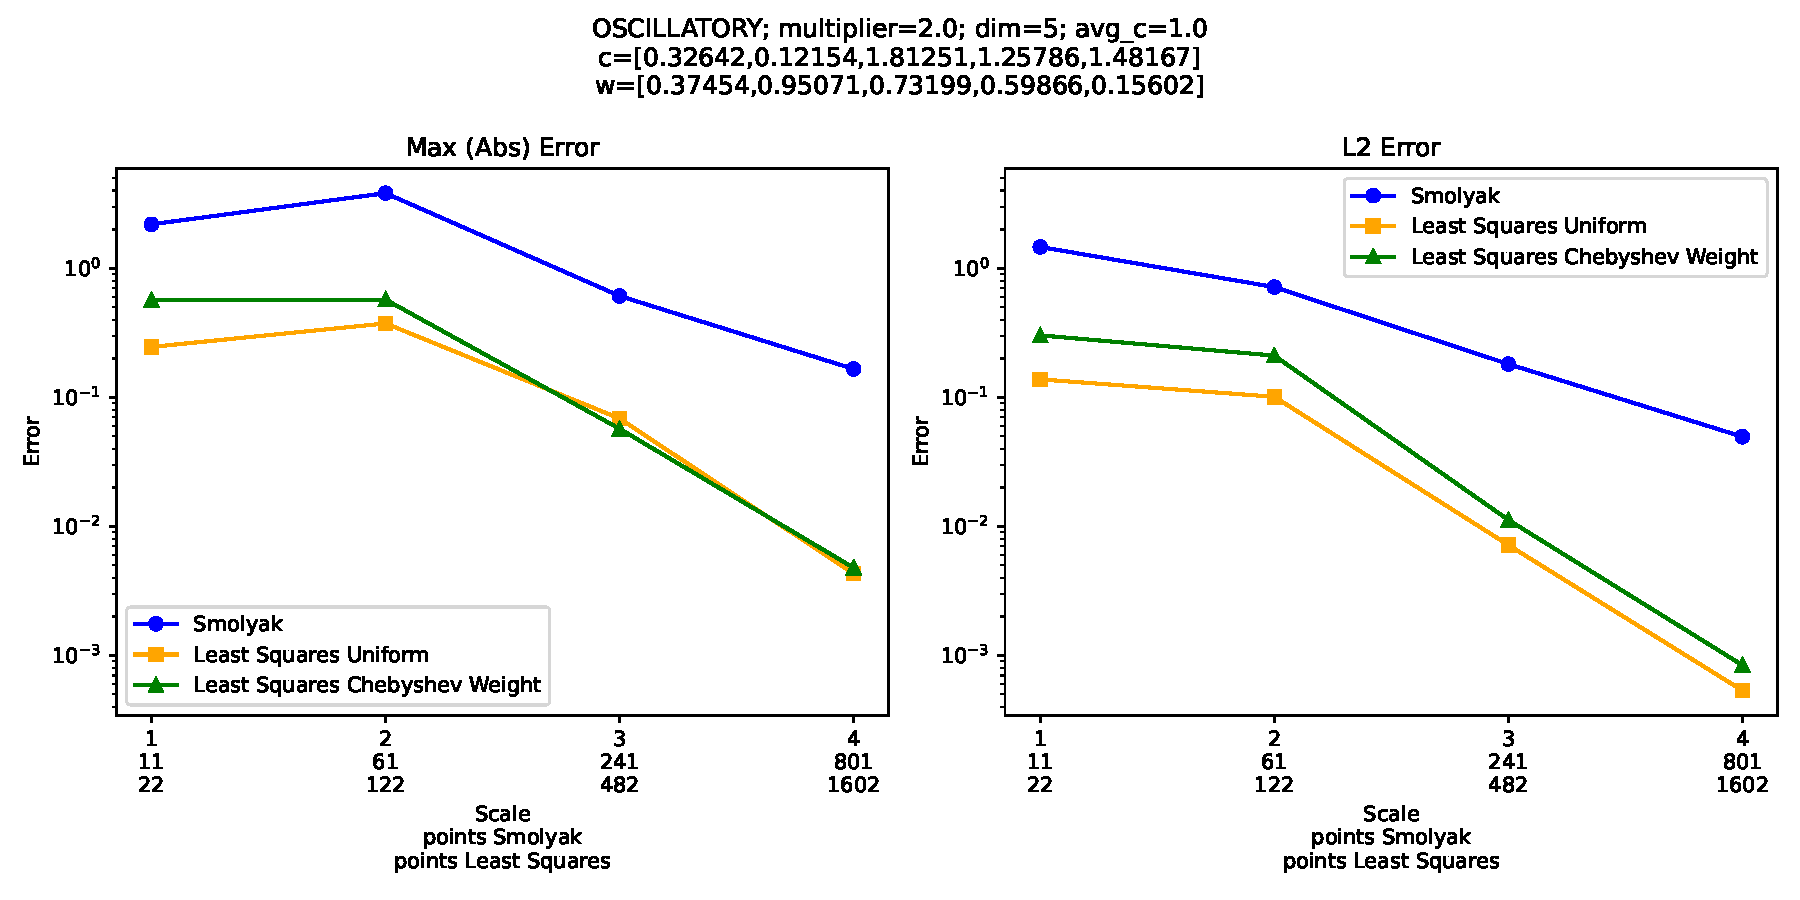
\includegraphics[width=\linewidth]{figures/oscillatory/realization1_dim5_scale4.pdf}
	\caption{Caption}
	\label{fig:Osc_1_dim5_scale4}
\end{figure}

\begin{figure}[H]
	\centering
	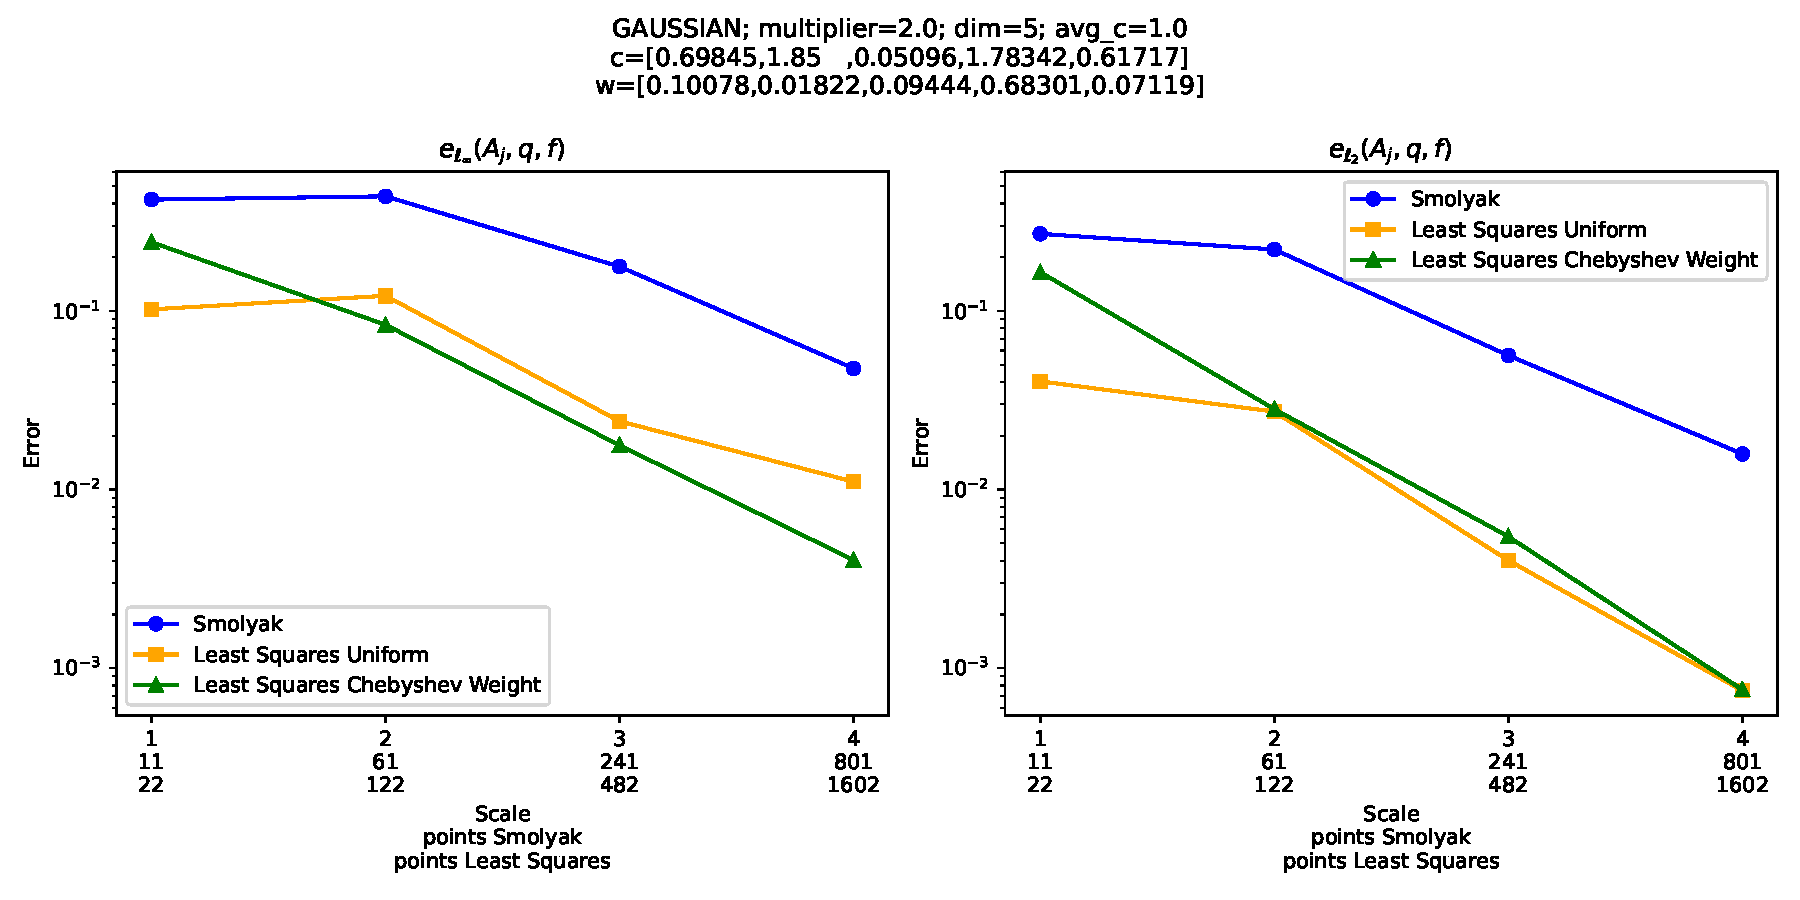
\includegraphics[width=\linewidth]{figures/oscillatory/realization2_dim5_scale4.pdf}
	\caption{Caption}
	\label{fig:Osc_2_dim5_scale4}
\end{figure}

\begin{figure}[H]
	\centering
	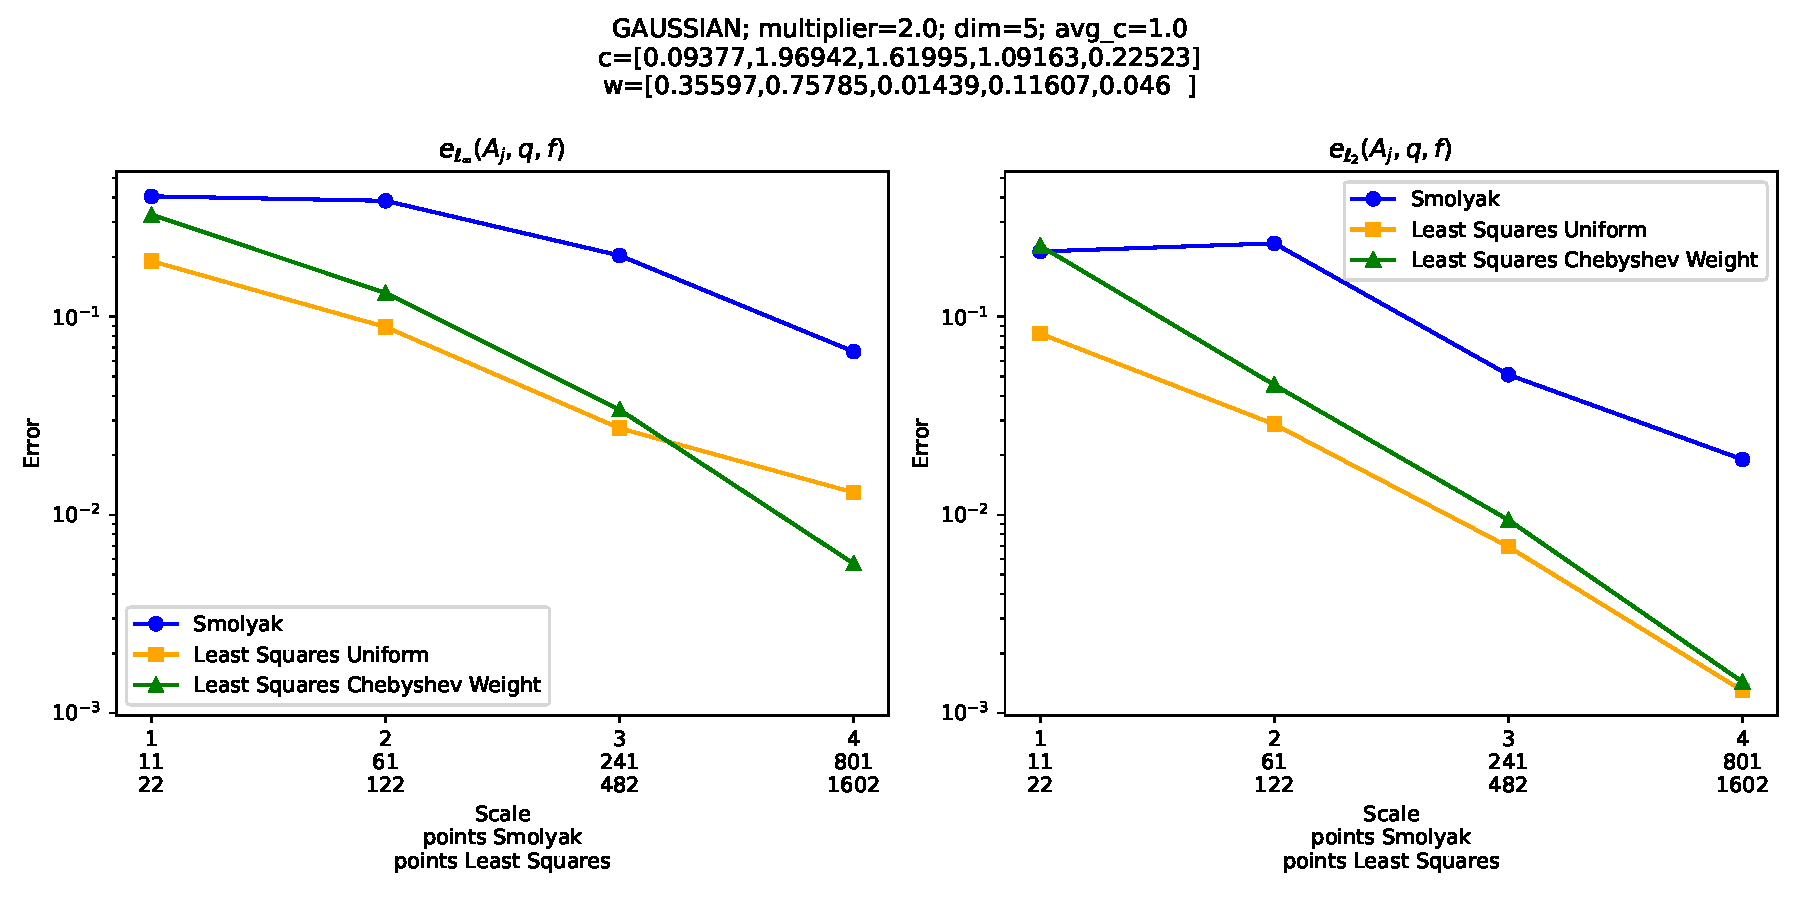
\includegraphics[width=\linewidth]{figures/oscillatory/realization3_dim5_scale4.pdf}
	\caption{Caption}
	\label{fig:Osc_3_dim5_scale4}
\end{figure}

\begin{figure}[H]
	\centering
	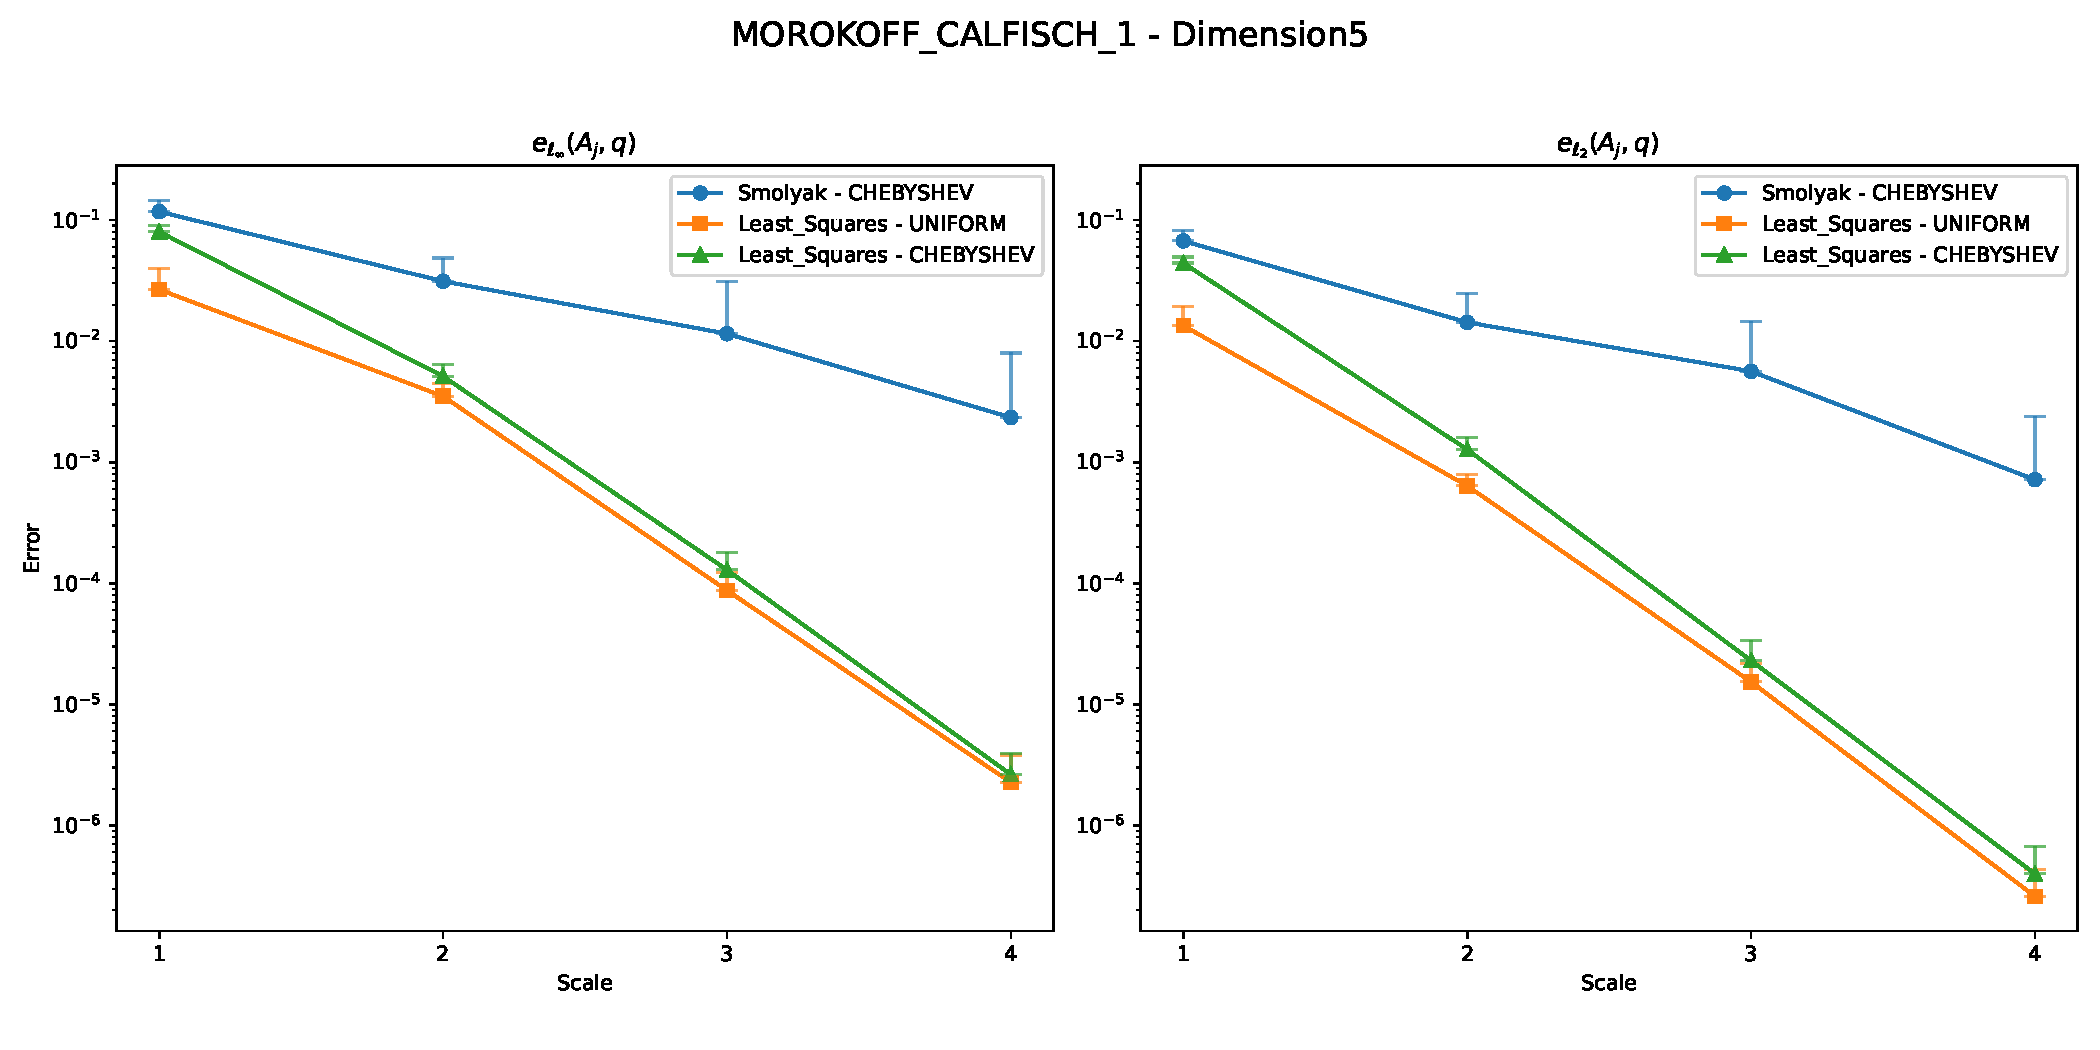
\includegraphics[width=\linewidth]{figures/morokoff_calfisch1/distro_dim5_scale4.pdf}
	\caption{Caption}
	\label{fig:morokoff_calfisch1_distribution_dim5_scale4}
\end{figure}

\begin{figure}[H]
	\centering
	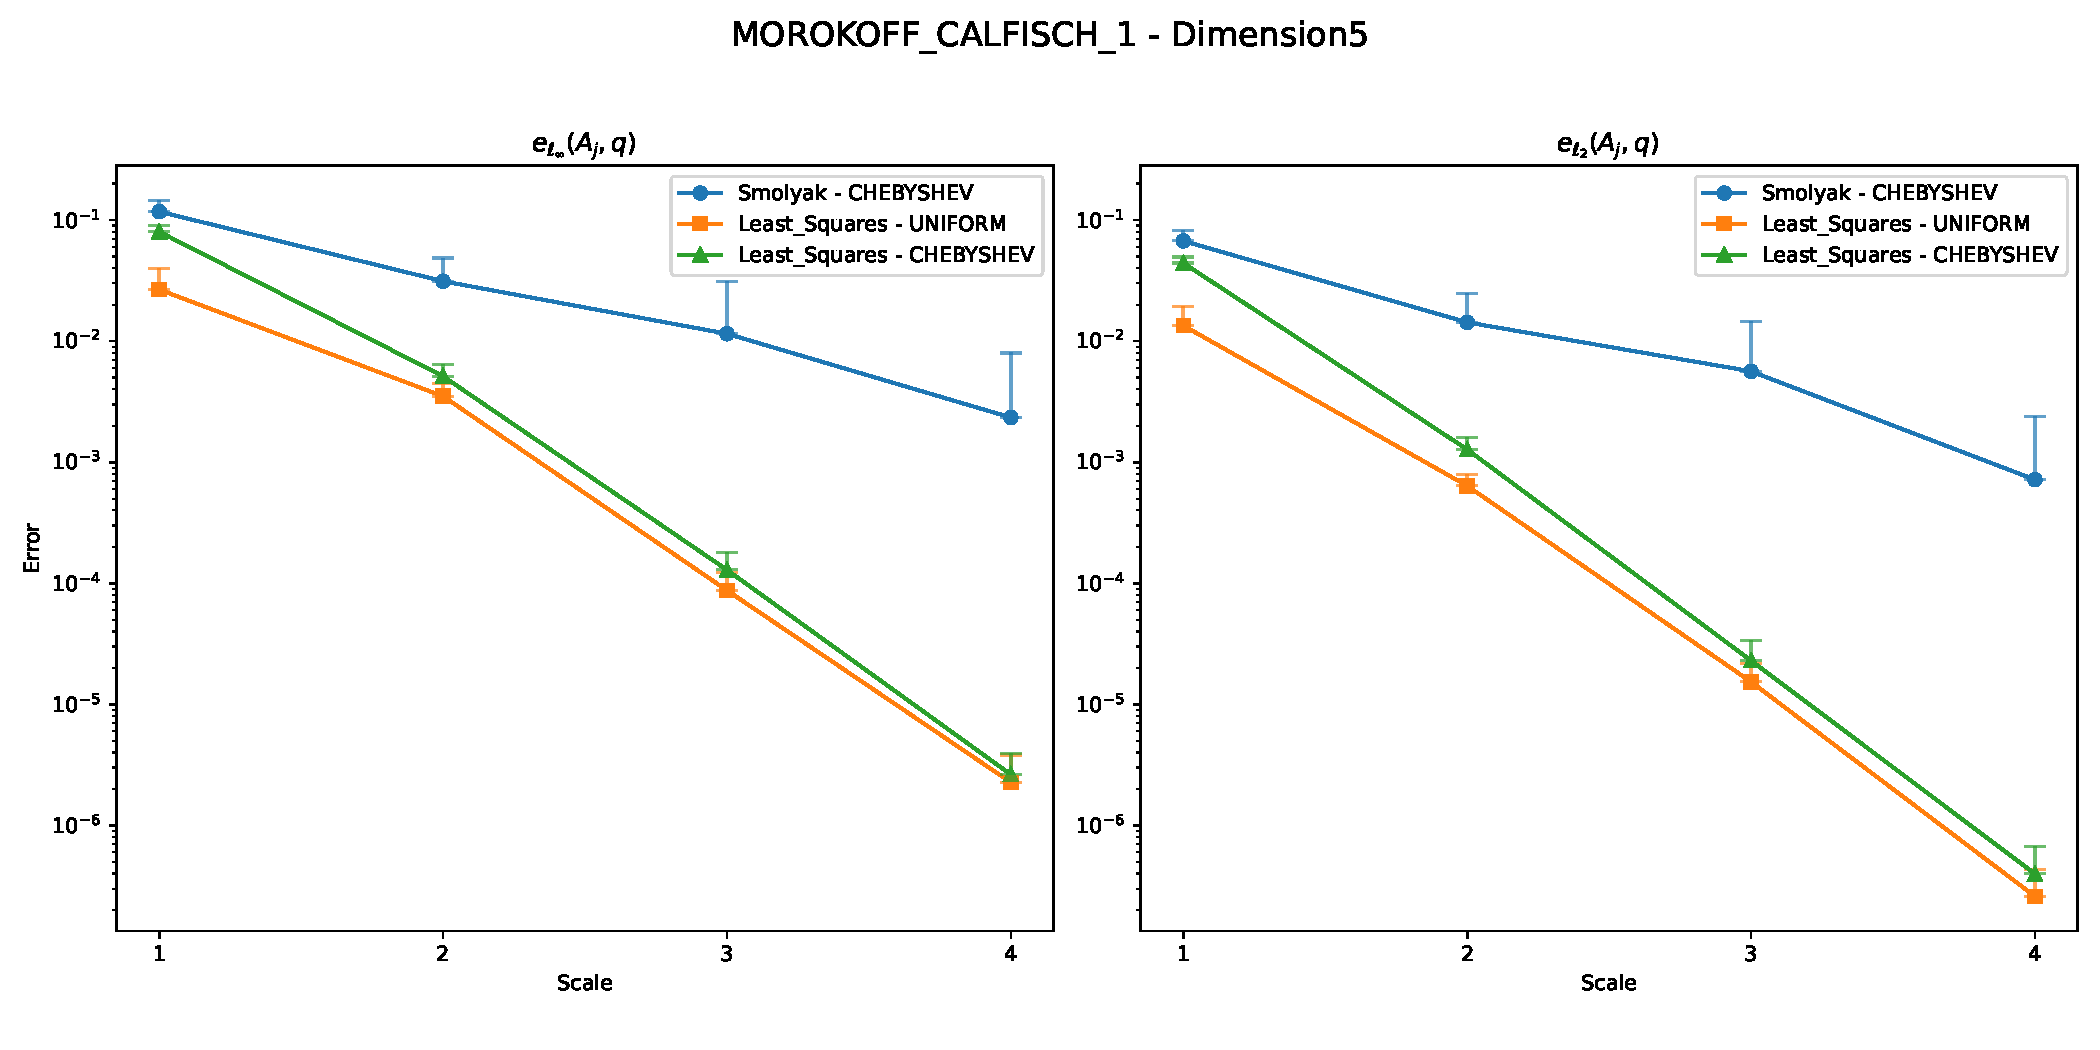
\includegraphics[width=\linewidth]{figures/morokoff_calfisch1/distro_dim5_scale4.pdf}
	\caption{Caption}
	\label{fig:morokoff_calfisch2_distribution_dim5_scale4}
\end{figure}

\begin{figure}[H] % TODO: Still with boxplot -> Maybe change
	\centering
	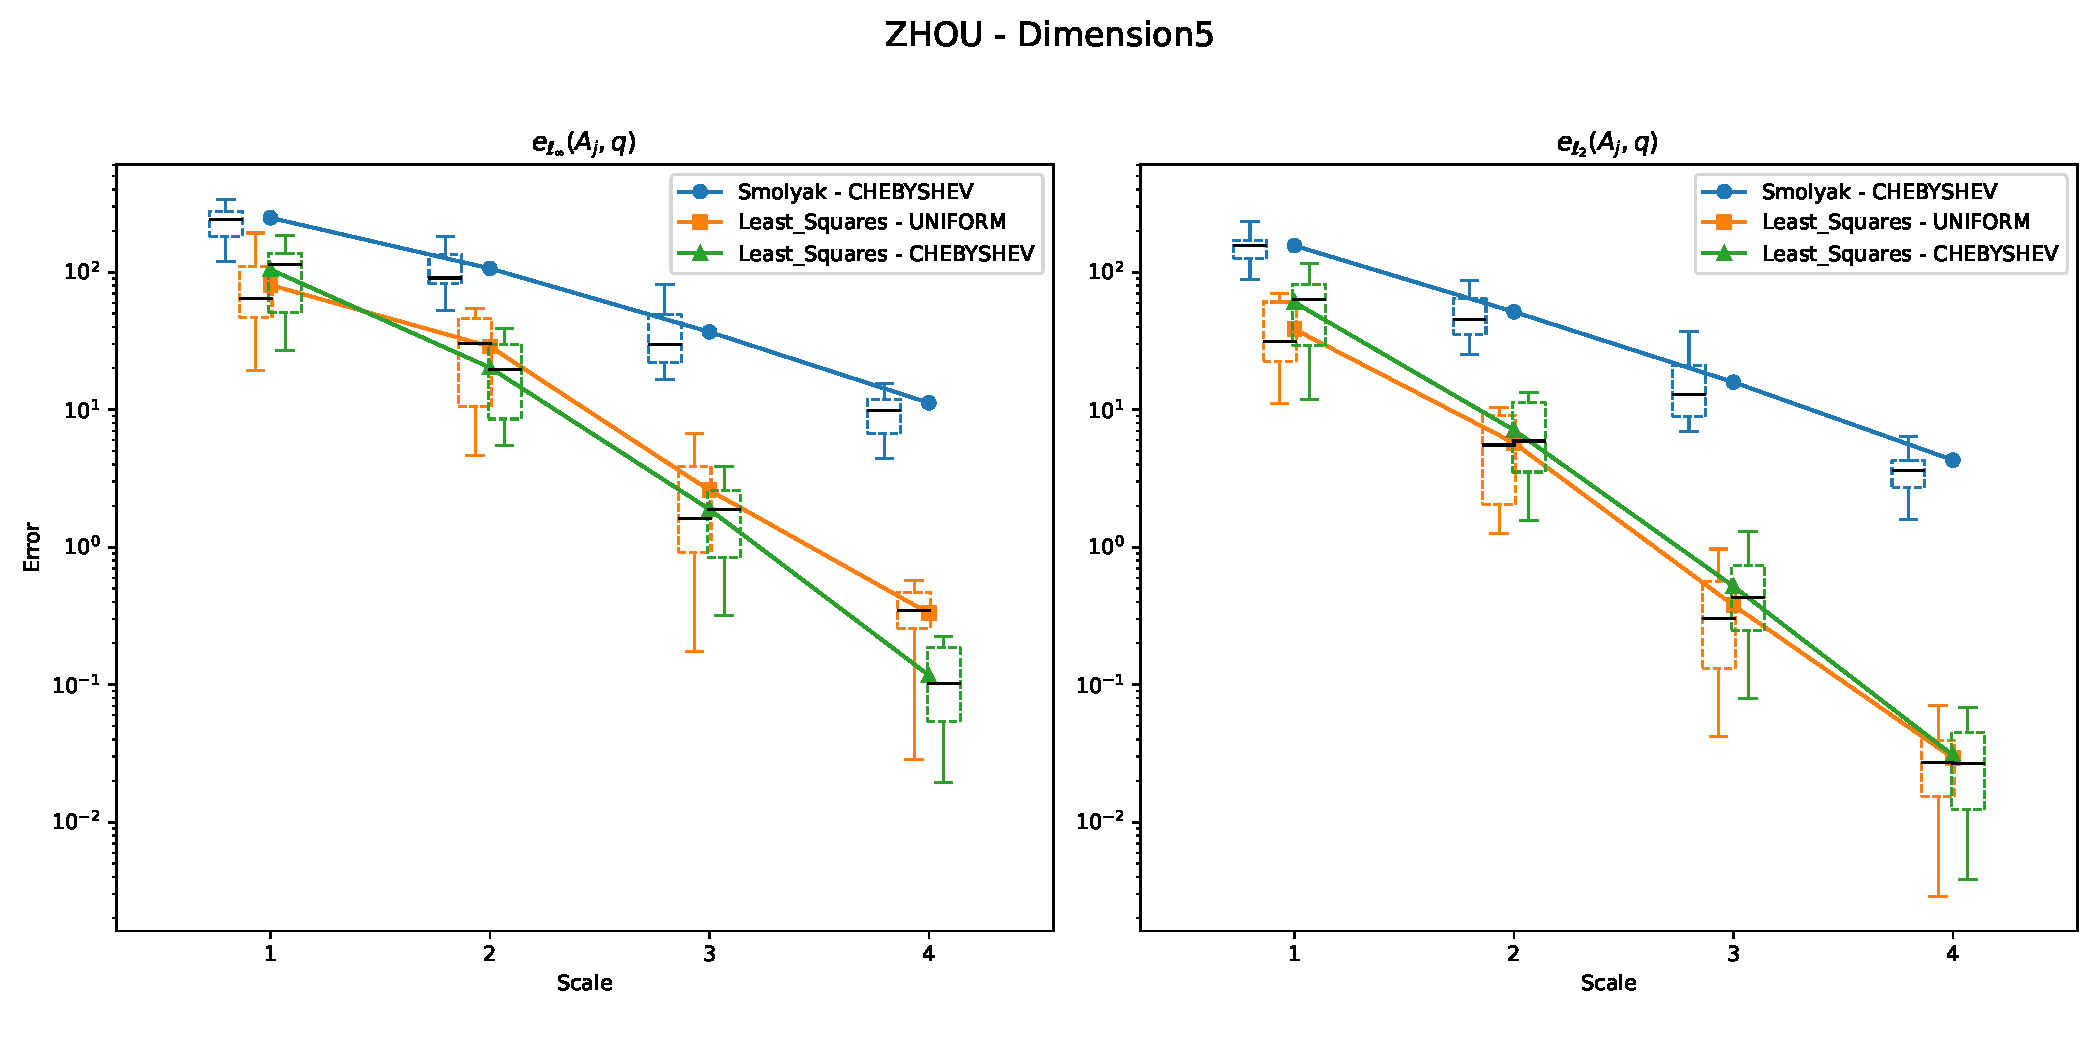
\includegraphics[width=\linewidth]{figures/zhou/distro_dim5_scale4.pdf}
	\caption{Caption}
	\label{fig:zhou_distribution_dim5_scale4}
\end{figure}



%%%%%%%%%%%%%%%%%%%%%%%%%%%%%%%%%%%%%%%%%%%%%%%%%%%%%%%%%%%
\section{Conclusion}\label{sec:conclusion}
%%%%%%%%%%%%%%%%%%%%%%%%%%%%%%%%%%%%%%%%%%%%%%%%%%%%%%%%%%%

% TODO: Write that down
Ideas
\begin{itemize}
	\item Same (or usually not a worse---mostly better) order of decay
	\item $2n$ points seem to suffice compared to the number of the paper
	\item In some cases, Least Squares outperforms Smolyak a lot
	\item Tasmainian: Sometimes bad performance: Bad implementation or maybe 
	sometimes Smolyak really bad (Mario: Approxing the $0$-Function). People 
	might not be aware of the fact that the approximation quality might be 
	extra-poor
	\item 
\end{itemize}


%%%%%%%%%%%%%%%%%%%%%%%%%%%%%%%%%%%%%%%%%%%%%%%%%%%%%%%%%%%
\section*{Acknowledgements}
%%%%%%%%%%%%%%%%%%%%%%%%%%%%%%%%%%%%%%%%%%%%%%%%%%%%%%%%%%%

% TODO: Maybe thank the Algebra Institute and RICAM for borrowing their cluster.
% TODO: Maybe thank other mathematicians for some comments and discussions 
	% TODO: (Mario has talked with some people I think)

% TODO: Richard Küng and Department for Functional Analysis for job?
% TODO: 


\newpage

\nocite{*}
\printbibliography

\bigskip

\noindent
% TODO: Mention the institue, and if yes, which one?
\address{J.E., Johannes Kepler University Linz; 
\texttt{jakob.eggl@jku.at}; \\
	E.M., Johannes Kepler University Linz; 
	\texttt{elias.mindlberger@jku.at}; \\
	M.U., Johannes Kepler University Linz; 
	\texttt{mario.ullrich@jku.at}
}

\end{document}
